%\section{Results}

\section{Building intuition}

% We start with building intuition about the characteristics of Brownian motion on an ARG using some simple toy examples. 

%There are two key advantages of a method that models stochastic movement on the full ARG. First, since the full ARG encodes information from every tree, we can estimate locations of genetic ancestors with higher certainty than a method that uses fewer trees. Second, the estimates of dispersal and location leverage information from the complete ARG structure, i.e., both the topology and the branch lengths. On the other hand, a peculiar characteristic of Brownian motion on an ARG is that, for a fixed number of samples every additional recombination event (as we increase the span of the genome under study) increases the dispersal estimate. We illustrate these points using simple ARGs first before working with simulations. 

\subsection{Ancestor locations}

% An ARG contains more nodes and branches than any single tree. Estimates under a model of Brownian motion are sensitive to this greater level of detail. 
Changing either the topology or branch lengths within an ARG will in general change the dispersal rate and ancestral location estimates. We show the latter in Figure \ref{fig:3samARG}, where we compare against two previous approaches: 1) The MLE of location with Brownian motion on each marginal tree \citep[as a heuristic for the likelihood method used in][]{osmond2024estimating} and 2) simple averaging, where a node's location is the average of its child nodes' locations \citep[as a heuristic for the method used in][]{Wohns2022}. By separately altering the timing of various nodes in the graph ($E$, $F$, and $G$), we observe a change in the MLE location of node $H$ under our model. In contrast, point estimates from the averaging method are unaffected by changes to node timing (green lines in Figure \ref{fig:3samARG}b), as this approach does not incorporate edge lengths. Meanwhile, a tree-based MLE (red and blue curves in Figure \ref{fig:3samARG}b) responds to changes in the timing of a node only if it affects the edge lengths in the given tree (e.g., the timing of node $G$ only affects shared times in the blue tree). Recombination nodes (e.g., node $F$) do not affect the shared times in trees as so their timing does not affect tree-based estimates. When the timing of a node affects a tree and is in a loop (e.g., node $G$), the ARG and tree estimates can show opposite trends (black vs.\ blue curves in Figure \ref{fig:3samARG}b-iii). Note that under a model of Brownian motion, moving node $G$ further into the past should move the location of node $H$ towards the locations of nodes $A$ and $B$ and away from the location of node $C$ (further explanation of this in ADD A REF TO SUPPLEMENT WHERE THIS IS EXPLAINED IN MORE DETAIL). This behavior is only captured when using Brownian motion on the ARG, not just on an individual tree.

\begin{figure}[ht]
    \centering
    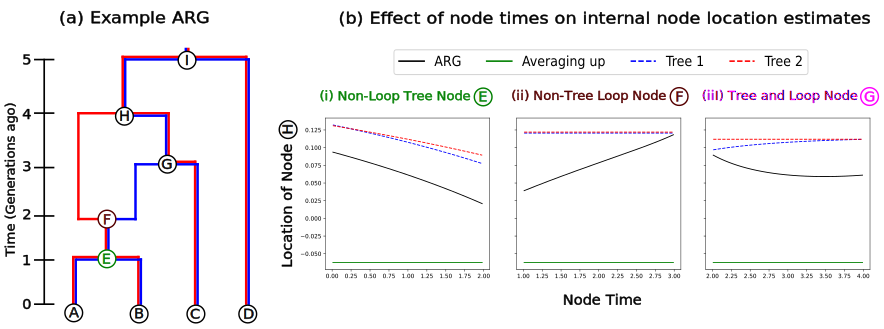
\includegraphics[width=\linewidth]{Images/Figure2_Topology/Fig2_TopologyEffects.png}
    \caption{\textbf{Ancestor locations}. (a) Toy 2-tree ARG. (b) Most likely location of node $H$ computed using the ARG (black), individual trees (red and blue), and the averaging-up method (green), plotted as a function of the time of (i) a node that alters individual trees and the ARG but is not part of the ARG loop, (ii) a node that doesn't alter individual trees but is part of the ARG loop and (iii) a node which is part of the ARG loop that alters a tree and the ARG. Locations of nodes $A$, $B$, $C$ and $D$ are -0.5, 0, 0.5 and 1, respectively.}
    \label{fig:3samARG}
\end{figure}

%The ARG method always estimated the location of node H to be closer to the locations of nodes A and B (placed at -0.5 and 0, respectively) compared to the estimates from either marginal tree (Figure \ref{fig:3samARG}B). This is due to the loop that is present between nodes F and H in the ARG; this loop constrains the dispersal along its edges. Intuitively, this can be reasoned as two lineages starting at the same point are more likely to meet if they didn't "wander" too far away from one another. Though initially believed to be a good property of this model, we will return to the consequences of this behavior when discussing dispersal rate inference in the next section.

%because the amount of time the path above node 2 spends in the loop is reduced, increasing the probability node 2 has moved further away. Only our method accurately captures this.

With the greater amount of information contained within the ARG vs.\ a single tree, we always estimate ancestor locations with higher certainty than the tree-based method provided we use the same dispersal rate (Figure \ref{fig:SingleLineage}c). In the absence of any other information, the variance in the location estimate increases linearly with time under Brownian motion. Both coalescent and recombination nodes bring additional information and hence reduce the increase in uncertainty of the location estimates as the lineage is tracked backwards in time (Figure \ref{fig:SingleLineage}c). Edges found across multiple trees, which are very common in large ARGs, show the greatest reduction in variance when using the ARG compared to a single tree.

\begin{figure}[hbtp]
    \centering
    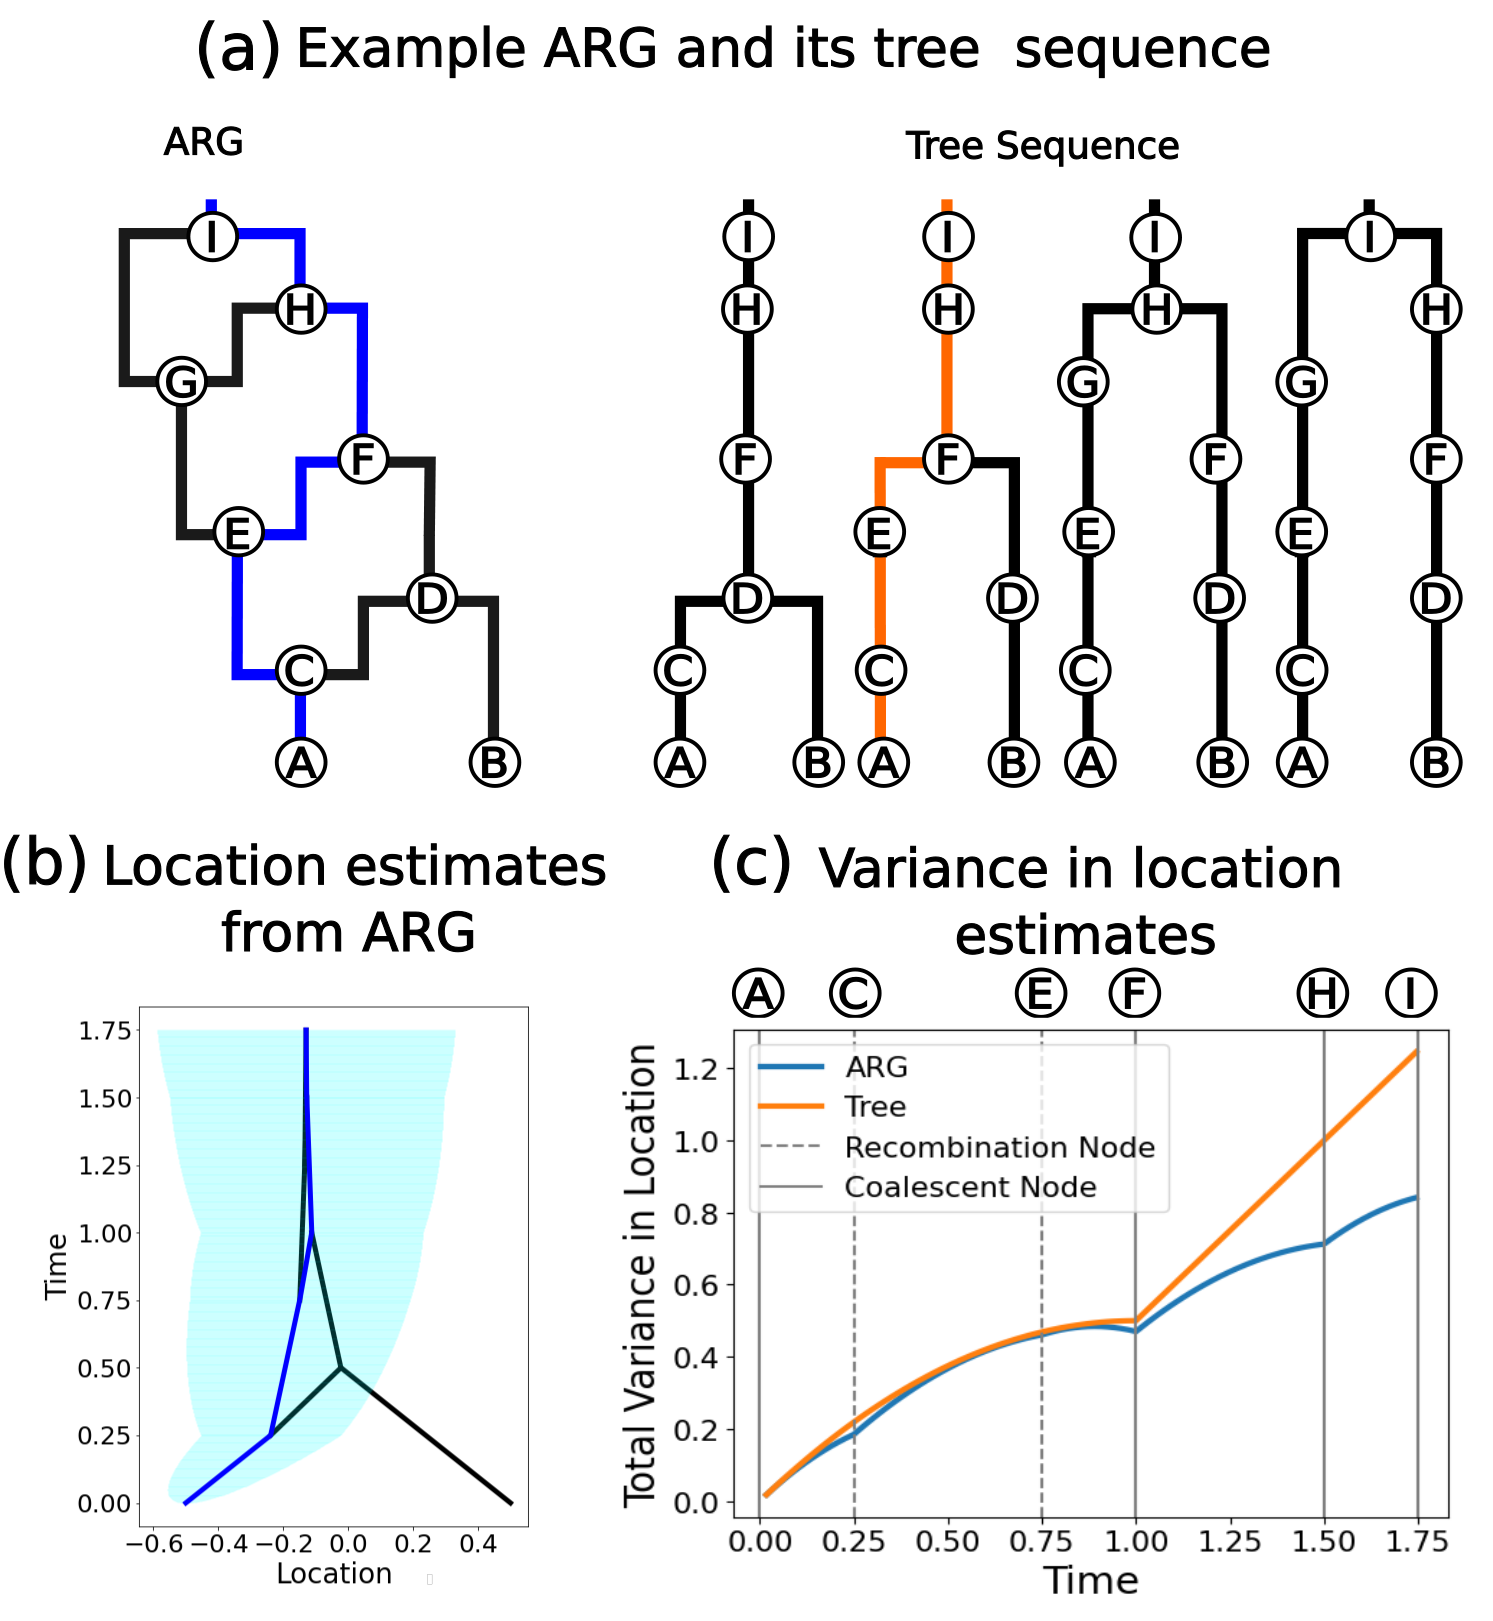
\includegraphics[width=\linewidth]{Images/Figure3_TrackLineage/Fig3_TrackSingleLineage.png}
    \caption{ \textbf{Uncertainty in ancestor locations}. (A) Example ARG and the corresponding tree sequence with the same path highlighted. (B) The most likely location estimates (lines) and the 95\% confidence interval of the blue path (shading) using the ARG. (C) The variance in location estimates, calculated using the true dispersal rates, along the highlighted path  using the full ARG (blue) and using just the single tree (orange).}
    \label{fig:SingleLineage}
\end{figure}

%Potentially counterintuitively, information coming in at these nodes can even lead to a reduction in uncertainty as you move backwards in time along an edge (e.g., the blue line between nodes 6 and 7 in Figure \ref{fig:SingleLineage}C). Altogether, ARGs incorporate more of the nodes, and so location estimates using the ARG will have smaller variances. 

%We show this in  using a simple 2-sample ARG consisting of four marginal trees.  

%Secondly, 


%an ARG-based approach like this leverages both the topology and branch lengths of the graph when estimating dispersal rate and ancestral locations. Figure \ref{fig:3samARG} shows that location estimates are sensitive these features.



%In Figure \ref{fig:SingleLineage}, we estimate the location of ancestors along a particular path through a 2-sample ARG consisting of four marginal trees. We show that the uncertainty (variance) in these location estimates is lower than the uncertainty of estimates from a model of Brownian motion on a single tree. In the absence of any other information, the variance in the location of a genetic ancestor increases linearly with time under Brownian motion. Both coalescent and recombination nodes reduce the increase in variance as they provide information that constrains the location estimate. Altogether, ARGs contain more of these nodes than are found in any individual tree within the graph; recombination nodes are not relevant for a single tree. Edges found across multiple trees have the greatest reduction in variance when using the ARG versus a single tree.

%In Figure \ref{fig:SingleLineage}, we estimate the location of ancestors along a particular path through a 2-sample ARG consisting of four marginal trees. We show that the uncertainty (variance) in these location estimates is generally lower than the uncertainty of estimates from a model of Brownian motion on a single tree. In the absence of any other information, the variance in the location of a genetic ancestor increases linearly with time under Brownian motion. In a tree, new information enters via coalescence events, which reduce the rate of increase in variance along edges below coalescence nodes (here the edge from 0 to 7). In an ARG, we generally see less uncertainty along a lineage because we get more coalescence events (here nodes 10 and 11) and we also get information coming in at recombination events (here nodes 2/3 and 5/6). Only along edges that only exist in a single tree (e.g.,,here from node 6 to 7) are the uncertainties from the ARG and the single tree potentially equal in some places. In practice, inferred ARGs will have many more samples than our toy example and so nearly every edge will exist in more than one tree. An ARG-based approach would then estimate ancestral locations with much more certainty than any single tree. %Note that when enough information comes in it is possible for the uncertainty in ancestor location to decline as we look back in time, using either trees or ARGs. Here we see such a decline at node 7 when using the ARG.We do not see this decline in uncertainty with the tree because less information comes in; the loop in the ARG reduces the uncertainty in the locations of ancestors along it.




%Figure \ref{fig:3samARG} shows that our location estimates are sensitive to both topology and edge lengths throughout the ARG. We compared our estimates to those from two previous approaches: 1) Brownian motion on each marginal tree \citep[as a heuristic for the likelihood method used in][]{Osmond2021} and 2) simple averaging, where a node's location is the average of its child nodes' locations \citep[as a heuristic for the method used in][]{Wohns2022}. Varying the timing of any other node affects our estimate for the location of node 8 (black curves in Figure \ref{fig:3samARG}B); changes like this ripple all  the way through the ARG. In strong contrast, the averaging method is completely insensitive to node timing (green lines in Figure \ref{fig:3samARG}B) as it does not use edge lengths. Meanwhile, the tree-based approach (red and blue curves in Figure \ref{fig:3samARG}B) captures changes in the time of a node that affects the edge lengths in a tree (e.g., node 4) but not of a node that leaves the trees unchanged (e.g., node 5/6). When the time of a node affects both the trees and is in a loop (e.g., node 7), the ARG and tree methods can show opposite trends. Note that, under our model, increasing the time of node 7 should move the location of node 8 towards the locations of nodes 0 and 1 and away from the location of node 2 because the amount of time the path above 2 spends in the loop is reduced, increasing the probability node 2 has moved further away. Only our method accurately captures this.

\subsection{Dispersal rate}

For a given number of samples, each additional recombination event in the ARG leads to a more clustered distribution of sample locations in the forward-in-time model. This means that, for a given set of sample locations, each additional recombination event in the ARG increases the dispersal estimate. We demonstrate the increased clustering of sample locations under the forward-in-time model in Figure \ref{fig:VarToy}. Focus on the variance in the location of the recombination node, $E$. First consider the two paths to $E$ ( $G \rightarrow E$ and $G \rightarrow F \rightarrow E$) independently. The variance of the location of $E$ along either path is $\sigma^2t$, where $t$ is the time between $G$ and $E$, which corresponds to the variances in the location of $E$ in each of the two the marginal trees. However, upon conditioning on the loop, $\eta_{loops}$, the variance in the location of $E$ reduces to half of its unconditioned variance, $\sigma^2 t/2$. More generally, we can treat the loop ($G \rightarrow E \rightarrow F \rightarrow G$) as a Brownian Bridge (REFERENCE), from $G$ back to $G$, and therefore calculate the variance at any point along the loop $X$ as $\frac{t_{X,G} (2t - t_{X,G}) }{2 t_{X,G}}$ where $t_{X,G}$ is the time between $X$ and $G$ (for instance, $t_{E,G} = t$). Intuitively, two lineages starting at the same point are more likely to meet again if they do not wander too far away from one another. This cascades down to reduce the variance of the sample locations below recombination nodes, leading to more clustered sample locations (see Appendix \ref{appendix:clusteringproof} for a proof and Figure \ref{fig:DispRate}c for simulations). 

This clustering also occurs, though to a lesser extent, in an alternate model of Brownian motion on an ARG \citep{Bastide2018}, which allows the parents of $E$ to be any distance apart and places $E$ at their midpoint (Figure \ref{fig:VarToy}b-iii). Here, for a single loop, the variance of the location of the recombination node is the variance in the average of its parents locations, $\text{Var}((\sigma^2t_{G,E} + \sigma^2t_{G,E})/2) = \sigma^2t_{G,E}/2$, just as in our original model. The difference is that, unlike the original model, the variance along the parental lineages (e.g., node $F$), and consequently the lineages branching off from those (node $C$), are not reduced. 

\begin{figure}[hbtp]
    \centering
    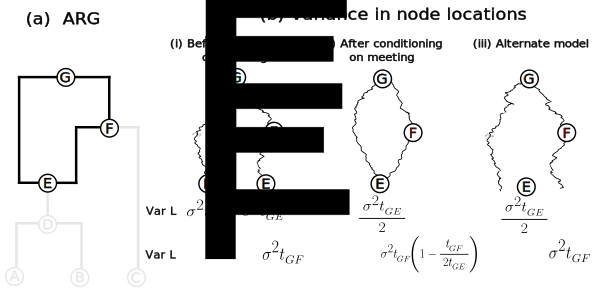
\includegraphics[width=\linewidth]{Images/Figure4_ToyVariance/Fig4_VarianceToyExample.png}
    \caption{\textbf{Variance in sample locations}. (a) The ARG with the loop highlighted. (b) The variances of nodes E and F of the loop (i) before conditioning on the two paths along the loop meeting at E, (ii) after conditioning on them meeting and (iii) for an alternate model, where E is located at the middle of the location of its two parents.   }
    \label{fig:VarToy}
\end{figure}


\section{Testing the theory}

\subsection{Simulations}

To assess the accuracy of estimates from this approach, we perform individual-based two-dimensional spatial simulations using SLiM v4.0 \citep{haller2023slim}, extending those run by \citet{osmond2024estimating}. Additional one-dimensional simulations and analyses are described in the supplementary materials (ADD REF TO SUPP). Simulations include density-dependent reproduction and a finite habitat boundary, both of which provide more realistic dynamics. Neither characteristic is captured directly under assumptions of Brownian motion, though \citet{osmond2024estimating} show that despite these differences, dispersal rates and ancestral locations can be accurately estimated under this model when applied to individual trees. Simulations start with 10,000 individuals uniformly randomly distributed in a $100 \times 100$ unit area, with each individual being diploid for a 1 megabase chromosome.  All individuals are hermaphrodites. In each generation an individual acts once as a mother, choosing its mate randomly based on distance (we assume a Gaussian mating kernel with variance $\sigma^2_m$) within a radius of $3\sigma^2_m$. The number of offspring for each mating pair is a Poisson random variable with mean $\lambda=\frac{2}{1 + C}$, where $C$ is the sum of the interaction strengths, also Gaussian with variance $\sigma^2_c$, with neighbors within a radius of $3\sigma^2_c$. When there are no mates within the interaction distance no offspring are produced. Offspring are placed relative to their mother's position with a normal random variable offset in each dimension with variance $\sigma^2_d$. If the offset would place the offspring outside of the area, the offset is reflected off of the boundary wall and back into the area. Note that the effective dispersal rate, the expected variance in the distance between the offspring and either parent not accounting for the reflections, is given by $\sigma^2_d + \frac{1}{2} \sigma^2_m$ \citep{smith2023dispersal}; the realized dispersal rate, accounting for the reflecting boundaries, will be lower. The locations and relationships between individuals are recorded in a tree sequence, which is saved at the end of the simulation \citep{haller2019tree}. Unless otherwise stated, the tree sequences are simplified to remove nodes that do not affect the broader topology of the graph and the ARG is chopped at 2000 generations in the past.

\subsection{Dispersal rate}
\label{dispersal_rate_section}

We first estimate dispersal rates from the simulated ARGs using Equation \ref{eq:sigmaMLE} and compare these estimates to the effective and realized dispersal rates from the simulations. We also compute the average dispersal rates calculated over the individual trees, which is identical to the composite likelihood method of \citet{osmond2024estimating} without importance sampling. Consistent with previous work \citep[e.g.,][]{kalkauskas2021sampling,Ianni2022}, the dispersal estimate from the composite likelihood over trees underestimates the simulated values (blue curve in Figure \ref{fig:DispRate}A) due to habitat boundaries. The average dispersal estimate over all trees stabilizes as we incorporate more trees (i.e., more of the chromosome). In contrast, the dispersal estimate from our ARG likelihood systematically increases as we include more trees, starting as an underestimate but eventually leading to an overestimate of the true dispersal rate (black curve in Figure \ref{fig:DispRate}A).

%We first used our method to estimate dispersal rates (Equation \ref{eq:sigmaMLE}) from simulated ARGs and compare these to dispersal estimates obtained from marginal trees \citep[using the composite likelihood-based method of][]{Osmond2021}. Unexpectedly, we fusingusingound that our ARG-based dispersal estimates were systematically biased. While disappointing, this highlights modeling issues arising from using Brownian motion models of dispersal that are worth understanding given that Brownian motion is a commonly used model. Despite the bias in the ARG-based estimate, we show that they more fully account for the uncertainty in our dispersal estimates compared to the composite likelihood estimate. This showcases an advantage of using the full ARG as opposed to a sequence of trees. 

%\subsubsection{Biased Estimates}

To understand the cause of this increase in the dispersal rate estimates under our model, recall that the displacements along edges in a loop are constrained as both sides of the loop need to come back together again. As we saw in the previous section, for a fixed dispersal rate the forward in time distribution of the sample locations becomes more clustered with more recombination nodes (simulations in Figure \ref{fig:DispRate}C and see Appendix \ref{appendix:clusteringproof} for a proof). Consequently, for a given set of sample locations, incorporating more trees into the ARG (and therefore more recombination nodes) must necessarily lead to a corresponding increase in the estimated dispersal rate. 
%To understand the cause of the systemic increase in dispersal rate estimate as we incorporate more trees along the genome, recall that the forward in time distribution of the tips becomes more clustered with more recombination nodes for a fixed dispersal rate. Consequently, for the same simulated sample locations, incorporating more trees (and therefore more recombination nodes) leads to an increase in the estimated dispersal rate. 
\begin{comment}
\begin{figure}[H]
\begin{subfigure}{0.33\textwidth}
    \caption{Dispersal Estimates}
    \includegraphics[width=\linewidth]{Images_Updated/Figure2/DispRateFinal.png}
\end{subfigure}
\begin{subfigure}{0.67\textwidth}
    \caption{Uncertainty in Estimates}
    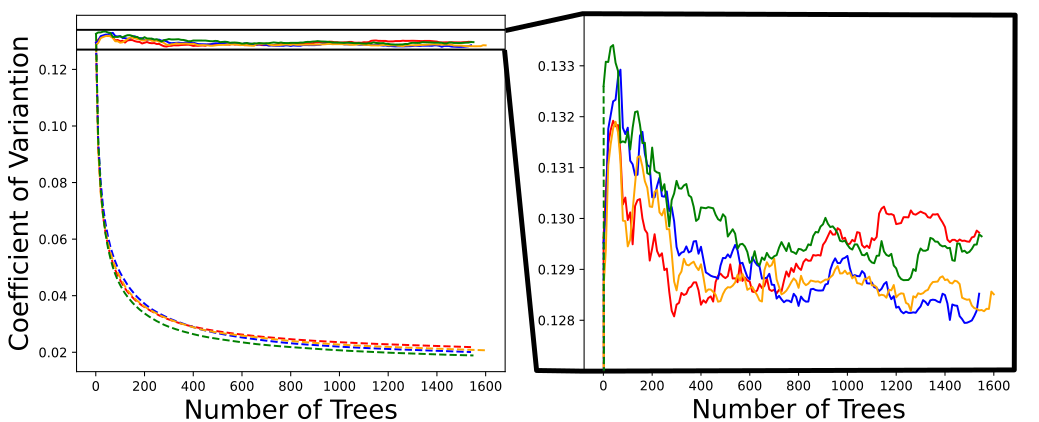
\includegraphics[width=\linewidth]{Images_Updated/Figure2/CoeffVarCombined.png}
\end{subfigure}

\begin{subfigure}{0.62\textwidth}
    \caption{Sample location distribution under different models}
    \includegraphics[width=\linewidth]{Images_Updated/Figure2/DispPattern_2000.png}
\end{subfigure}
\begin{subfigure}{0.37\textwidth}
    \caption{Complementary Simulations}
    \includegraphics[width=\linewidth]{Images_Updated/Figure2/DispRateCheck.png}
\end{subfigure}
\caption{\textbf{Dispersal rate}. (A) Dispersal rate estimates as a function of the number of trees used. We compare the maximum composite likelihood estimate over trees (blue), the maximum composite likelihood estimate over trees after fixing the node locations according to the ARG (green), and the full ARG maximum likelihood estimate (black). (B) The coefficient of variation in the dispersal rate when computed using the composite likelihood over trees (dashed) and the ARG likelihood (solid) as a function of the number of trees used. Each color is an independent replicate. (C) The expected distribution of sample node locations under three different models. } \label{fig:DispRate}
\end{figure}
\end{comment}
\begin{figure}[H]
\begin{subfigure}{0.32\textwidth}
    \caption{Dispersal Estimates}
    \includegraphics[width=\linewidth]{Images/Figure5_DispersalRate/DispRateFinal.png}
\end{subfigure}
\begin{subfigure}{0.32\textwidth}
    \caption{Effect of \\ Mating Distance}
    \includegraphics[width=\linewidth]{Images/Figure5_DispersalRate/DispRateMating.png}
\end{subfigure}
\begin{subfigure}{0.32\textwidth}
    \caption{\centering Effect of \\ local competition}
    \includegraphics[width=\linewidth]{Images/Figure5_DispersalRate/DispRateComp.png}
\end{subfigure}
\begin{center}
\begin{subfigure}{0.75\textwidth}
    \caption{\centering Sample location distribution under different models}
    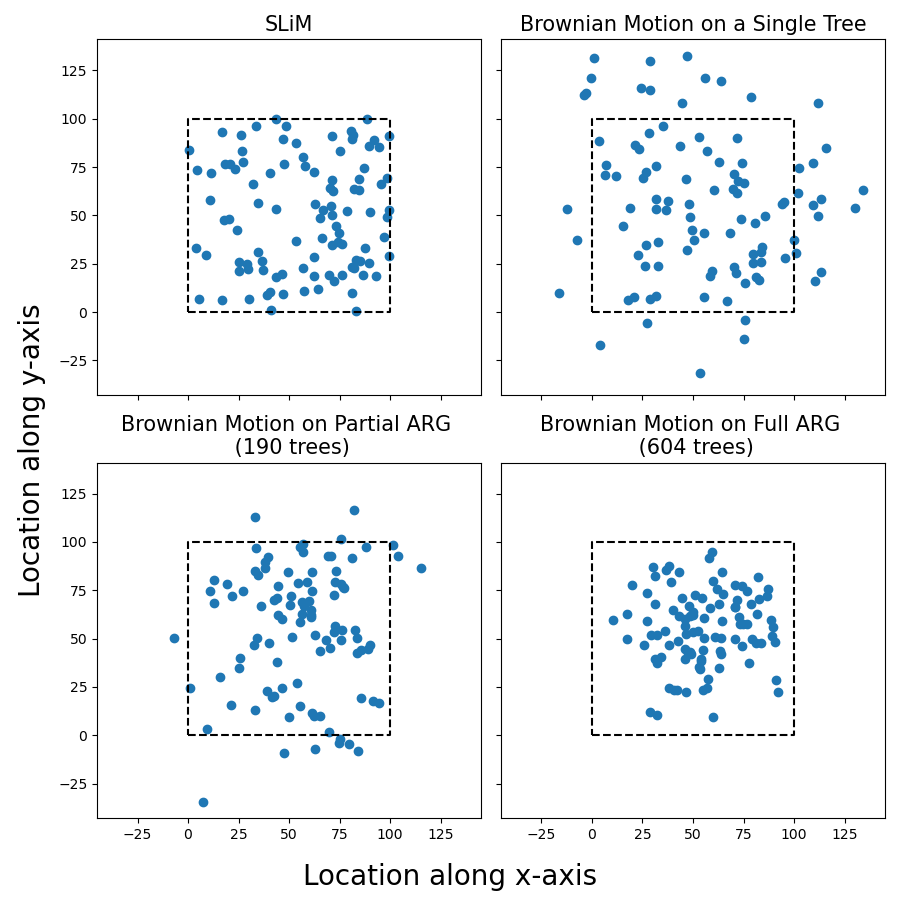
\includegraphics[width=\linewidth]{Images/Figure5_DispersalRate/DispPattern.png}
\end{subfigure}    
\end{center}

\caption{\textbf{Dispersal rate accuracy}. (a) Dispersal rate estimates as a function of the number of trees used in the computation. We compare the maximum composite likelihood estimate over marginal trees (blue) and the maximum likelihood estimate of the ARG composed of the same set of trees (black). The dashed line is the effective dispersal rate (averaged over maternal and paternal variances) used in the simulation. The dashed-dotted line is the realized dispersal rate in the simulation (average squared displacement per time over all edges), which accounts for habitat boundaries.
(b-c) Full ARG maximum likelihood dispersal estimates as a function of the number of trees colored by the variance in the (b) mating kernel and (c) competition kernel (5 replicates each).(d) The expected distribution of sample node locations under four different models. In the top left we show the sample locations from a replicate of the individual-based simulation. We then use this simulated ARG to draw sample locations from a model of Brownian motion down a single tree (top right), down a portion of the ARG (bottom left), and down the full ARG (bottom right). The dotted line is the habitat boundary of the SLiM simulations.  } \label{fig:DispRate}
\end{figure}


To confirm that conditioning on lineages meeting at the recombination nodes is the core cause of the bias in dispersal rate estimates, we next run simulations that are closer to Brownian motion. The original SLiM simulations differ from Brownian motion in two main aspects: 1) they allow some distance between mates and 2) they have local density regulation. We address these separately. First, we decrease the average mating distance by reducing the variance of the mating kernel, $\sigma^2_m$ (Figure \ref{fig:DispRate}b). Second, we make density regulation more global by increasing the variance of the competition kernel, $\sigma^2_c$ (Figure \ref{fig:DispRate}c). Less localized competition leads to more clumping due to the ``pain in the torus" \citep{Felsenstein1975} and therefore indirectly decreases the average distance between mates. As a result, both of these modifications reduce the error in dispersal rate estimates and cause them to increase more slowly with the number of trees (Figure \ref{fig:DispRate}d).

%In one set of simulations we by simulating scenarios with (i) reduced distance between mates by reducing the variance of the mating kernel, $\sigma^2_m$ (Fig \ref{fig:DispRate} b) and (i) less localized competition by increasing the variance of the competition kernel, $\sigma^2_c$ (Fig \ref{fig:DispRate} c). Less localized competition leads to more clumping due to the "pain in the torus" \citep{Felsenstein1975} and therefore to a lower realized distance between mates. As a result, both (i) and (ii) brought the dispersal rate estimates closer to simulated value. Further, the dispersal estimates increased less quickly with the number of trees (Figure \ref{fig:DispRate}d).

We can also investigate the cause of the dispersal rate bias by modifying our model of inference. A key assumption is that we force parent lineages to meet exactly at recombination nodes. We completely relaxed this assumption by allowing parents to mate from any distance and placing the recombination node at their midpoint (Appendix \ref{appendix:RelaxedBM}). However, because the variance of the recombination node is reduced to a similar extent as in the original model (Figure \ref{fig:VarToy}b), we still see an increase in dispersal estimates as we increase the number of trees (Appendix \ref{appendix:RelaxedBM}). But, unlike the original model, the variance along the parental lineages (e.g., node $F$ in Figure \ref{fig:VarToy}b-iii), and consequently the lineages branching off from those (node $C$), are not reduced. This reduces the rate at which the dispersal estimate increases with the number of trees (Appendix \ref{appendix:RelaxedBM}).

%Second, we use the original Brownian motion model but restrict to windows along the genome, i.e., we split the genome into shorter disjoint segments and compute the composite likelihood over the segments (see \cite{Larribe2011} and \cite{Meligkotsidou2007} for previous uses of composite likelihood in genetics). This gets rid of the monotonic increase in dispersal with the span of the genome under consideration, since each segment has a similar number of recombination events (Fig \ref{appendix:RelaxedBM}). 

\begin{comment}
\begin{figure}[h]
\begin{subfigure}{0.45\textwidth}
    \caption{Varing Mating Distance}
    \includegraphics[width=\linewidth]{Images_Updated/Figure3/DispRateMating.png}
\end{subfigure}
\begin{subfigure}{0.45\textwidth}
    \caption{Varying degree of local competition}
    \includegraphics[width=\linewidth]{Images_Updated/Figure3/DispRateComp.png}
\end{subfigure}

\caption{Dispersal Rate Estimates for different values of (a) the variance of mating distance $\sigma^2_m$ and (b) the variance of the interaction distance $\sigma^2_c$} \label{fig:DispRate}
\end{figure}

\begin{figure}[ht]
    \centering
    \includegraphics[width=\linewidth]{Image/Fig3_DispersalRate.jpg} 
    \caption{\textbf{Dispersal rate}. (A) Dispersal rate estimates as a function of the number of trees used. We compare the maximum composite likelihood estimate over trees (blue), the maximum composite likelihood estimate over trees after fixing the node locations according to the ARG (green), and the full ARG maximum likelihood estimate (black). (B) The coefficient of variation in the dispersal rate when computed using the composite likelihood over trees (dashed) and the ARG likelihood (solid) as a function of the number of trees used. Each color is an independent replicate. (C) A toy 2-tree ARG (left). The most likely locations of ancestors given the sample locations (middle) for the two  trees (red and blue) when computed independently (dashed) and when computed using the ARG (solid). Dispersal rates estimates (right) assuming node locations in the two trees are independent (composite) or a compromise (ARG).} \label{fig:DispRate}
\end{figure}


There are two main reasons for the systematic increase in the ARG dispersal rate, both of which arise, mathematically speaking, because of how the MLE dispersal rate under Brownian motion is calculated, by first choosing internal node locations to minimize the displacements that descendent nodes need to disperse. The MLE dispersal rate is then the average squared displacement over edges, 
\begin{eqnarray}
    \displaystyle \hat{\sigma^2} = \min_{\text{node locations}}\frac{1}{n} \sum_{\text{edge in ARG}} \frac{D_{edge}^2}{t_{edge}},
    \label{eq:arg}
\end{eqnarray}
where $n$ is the number of edges and $D_{edge}$ and $t_{edge}$ are the displacement and length of an edge \citep{maddison1991squared}. We can then understand the ARG dispersal bias as coming from two factors:

\begin{enumerate}

    \item \textbf{Compromising ancestral locations  across trees}. When trees are treated independently, e.g., under the composite likelihood estimate of dispersal, the node locations in each tree can be independently chosen to minimize the displacements (the set of $D_{edge}$ for each tree). However, the nodes within an ARG are often shared across multiple trees, and so the choices of node locations must minimize the dispersal distances across all of the trees together rather than any tree individually. This ultimately leads to higher dispersal rates for each tree. To demonstrate this we recalculated the composite likelihood dispersal rate but now with each individual tree's node locations computed from the ARG ("constrained composite likelihood") and found it to be higher than when each tree's node locations are minimized independently (see toy example in Figure \ref{fig:DispRate}C). Further, the more trees represented in the ARG, the greater the constraint, leading to higher dispersal rates for each tree and consequently a higher average (green curve in Figure \ref{fig:DispRate}A) compared to the (unconstrained) composite likelihood (blue curve in Figure \ref{fig:DispRate}A). Thus, the compromise over node locations within the ARG partly explains why the ARG dispersal estimate is higher than the composite likelihood estimate over trees and why it increases with the number of trees (more trees lead to more constraint), but it does not fully explain the issue, as the constrained composite likelihood dispersal rate is lower than the ARG dispersal rate (black curve in Figure \ref{fig:DispRate}A).  

    \item \textbf{Averaging dispersal rates over trees}. To understand why the ARG dispersal estimate is greater than even the constrained composite likelihood estimate, note that constrained composite likelihood estimate is the average dispersal estimate over all trees,
    \begin{eqnarray}
        \hat{\sigma^2}_{constrained} = \frac{1}{\# \text{trees}}\sum_{\text{tree}} \frac{1}{n} \sum_{\text{edge in tree}} \frac{D_{\text{edge}}^2}{t_{\text{edge}}},
        \label{eq:average_arg}
    \end{eqnarray}
    where the displacement over the edge, $D_{\text{edge}}$, is calculated from node locations inferred from the full ARG (Equation \ref{eq:arg}). Now, an edge that exists in every tree would contribute the same amount to the constrained composite estimate (Equation \ref{eq:average_arg}) as it would to the ARG estimate (Equation \ref{eq:arg}), but an edge that belongs to fewer trees will contribute less to the constrained estimate (Equation \ref{eq:average_arg}). Consequently, the more trees that we include in the ARG, the greater the number of edges that are not shared by all trees. Hence, the constrained composite likelihood estimate does not increase as quickly as the ARG estimate. That said, the averaging in the composite likelihood (Equation \ref{eq:average_arg}) is not the right approach as it ignores the non-independence of the trees. Intuitively, each edge in the ARG should be given equal weight while computing the dispersal rate, justifying the ARG estimate (Equation \ref{eq:arg}) under the assumption of Brownian motion. While the ARG estimate may be better justified from a statistical perspective, the mis-specification of Brownian motion as a model of dispersal generates significant biases. 
    
\end{enumerate}

We next propose two methods that reduce the compromise across the trees. Both methods have better properties with respect to dispersal estimates. 
\begin{enumerate}
    
    \item \textbf{Windowing}. Using a subset of adjacent trees from the ARG reduces the compromise in ancestral locations. This preserves the key benefits of our method, that is, using the full likelihood over multiple trees and the computational efficiency of the minimal paths algorithm. To calculate the dispersal rate we can split the genome into a series of non-overlapping windows and take the composite likelihood over these. The downside of this approach is that we ignore the correlations between trees in different windows (but see, for e.g., \cite{Larribe2011} and \cite{Meligkotsidou2007} for previous uses of composite likelihood in genetics). The resulting dispersal estimate asymptotes with the number of trees at a larger value than the composite likelihood estimate, as there are still some compromises in node locations (red curve in Figure \ref{fig:S_DispersalRate}).
    
    \item \textbf{Relaxed Meeting}. Instead of forcing parental lineages to precisely meet at a recombination node, we explore the other extreme and allow the two parents of a recombinant offspring to be any distance from each other, placing the offspring at their midpoint (Appendix \ref{appendix:RelaxedBM}). Doing this allows adjacent trees to adjust the locations of their non-shared nodes more freely. The resulting dispersal estimate increases more slowly than the constrained composite likelihood with the number of trees (Figure \ref{fig:S_DispersalRate}) and sometimes decreases. Unfortunately, the dispersal estimate still increases on average and is more computationally expensive since we need to use the Full Paths Matrix instead of the Minimal Paths Matrix. 
    
\end{enumerate}
\end{comment}
 

\subsection{Ancestor locations}

To assess the accuracy of estimated ancestor locations (Equation \ref{eq:Lint}), we estimate the location of random genetic ancestors within a simulated ARG of 1000 samples and compare to the truth. We select each genetic ancestor to locate by choosing a random sample, genome position, and time (e.g., the ancestor of sample 1 at genome position 1050bp, 200 generations in the past). We estimate a location using the ARG for the full chromosome ("ARG"), a local ARG containing 100 trees on either side of the chosen genome position ("Window 100"), and the local tree at the genome position ("Tree"). We also compare these estimates against those using the averaging-up approach \citep{Wohns2022}. For the averaging-up method, we first simplified our ARG before calculating the locations \citep{Kelleher2018, Wong2023}, as is done in practice \citep{Wohns2022}.

Despite using more information, we observe larger absolute error with the full chromosome ARG estimates than with the tree-based approach (Figure \ref{fig:ancestral_locations_plots} left). Drilling into this further, we see that ancestors are often estimated too close to the average ("center") of the sample locations (Figure \ref{fig:ancestral_locations_plots} middle). Since the forward-in-time model sees excess clustering below recombination nodes (Figure \ref{fig:VarToy}b-ii, Figure \ref{fig:DispRate}d), backwards in time there is an equivalent pull towards the center. This bias towards the center becomes more severe as more trees are incorporated into the ARG.  
Perhaps surprisingly, we see that the averaging-up method, which uses a simplified ARG and ignores edge lengths, performs just as well on average. 

Lastly, we see that the average uncertainty in location estimates gets smaller as we use more trees (Figure \ref{fig:ancestral_locations_plots} right). The uncertainties depend on the dispersal estimate. We used the true dispersal rates to understand the unique properties of the location uncertainties, distinct from the issues of the dispersal estimate. This is in part because each tree brings in more information, increasing our certainty in inferred ancestor locations. However, with more trees the model eventually becomes overconfident, underestimating uncertainty (REF our coverage plot, now in sup mat?). Local ARGs may therefore be a promising direction forward; the number of trees incorporated into the local ARG may be chosen so that the mean error is no worse than that from a single tree or the averaging-up method (Figure \ref{fig:ancestral_locations_plots} left) and the uncertainty is more accurate (REF coverage plot). However, there is currently no way of determining an appropriate number of trees to use in the local ARG. 

% In other simulations (not shown), we see that this pattern is dependent on the number of samples in the ARG; occasionally, you can even have greater uncertainty with the ARG estimates than those using a single tree. This is due to the bias in the dispersal rate, which is a major component of the estimate variance/uncertainty (Equation \ref{eq:VarLint}).



%also display a bias towards the center of the sample locations.

%We calculated the error between estimates of the most likely location of an ancestor and its true location (Figure \ref{fig:ancestral_locations_plots}A). Interestingly, we see that the average error of our method increases as we use more trees (increasing window size). This turns out to be caused by an increasing bias in ancestral locations estimates towards the average sample location (Figure \ref{fig:LocationErrorBias}). As we explained in the dispersal section above, including more trees leads to more compromises in internal node locations, generally pushing them faster towards the average sample location. While the internal node locations should generally converge to the average sample location eventually, the compromises imposed  by our model are too strong and as a result the window size with the lowest average error is a single tree. Perhaps surprisingly, we see that the relatively simple averaging-up method, which uses a simplified ARG and ignores edge lengths, performs just as well on average.



%Closely tied to the patterns that we observe in dispersal rate estimates, estimates of ancestral location using Equation \ref{eq:Lint} also display a bias towards the center of the sample locations. Lineages are quickly drawn 

%To illustrate the implications of using the ARG for locating genetic ancestors, we first to a simple ARG (Figure \ref{fig:3samARG}A) and compare our estimate of the most likely location of node 8 to 1) the estimate from each marginal tree \citep[as a heuristic for the likelihood method used in][]{Osmond2021}  and 2) the estimate from a simple averaging method, where a node's location is the average of its child nodes' locations \citep[as a heuristic for the method used in][]{Wohns2022}.

%\subsubsection{Using More Information}

%Our method uses the structure and edge lengths from the full ARG and in doing so captures more information than existing methods. To illustrate the implications of this for locating genetic ancestors, we apply our method to a simple ARG (Figure \ref{fig:3samARG}A) and compare our estimate of the most likely location of node 8 to 1) the estimate from each marginal tree \citep[as a heuristic for the likelihood method used in][]{Osmond2021}  and 2) the estimate from a simple averaging method, where a node's location is the average of its child nodes' locations \citep[as a heuristic for the method used in][]{Wohns2022}. 

% Similar to the tree method, but unlike the averaging method, our method captures the effect of varying the time of a node that changes tree and ARG edge lengths but does not belong to a recombination loop (Figure \ref{fig:3samARG}B left). In addition, our method captures the effect of varying the time of a node in a recombination loop that does not affect individual tree edge lengths but does change the ARG edge lengths, an effect which none of the other methods capture (Fig \ref{fig:3samARG} middle ). Finally, the effect of varying the time of a node that is part of a recombination loop and alters at least one tree's branch lengths tends to go in the opposite direction between our method and the tree method  (\ref{fig:3samARG} right). Note that, intuitively, increasing the time of node 7 should move the location estimate of node 8 towards the locations of nodes 0 and 1 because the amount of time the path above 2 spends in the loop is reduced, increasing the probability node 2 has moved further away.  

%Our method captures the effect of varying the time of any node (black curves in Figure \ref{fig:3samARG}B). In contrast, the averaging method is insensitive to the time of any node as it does not use edge lengths (green lines in Figure \ref{fig:3samARG}B). Meanwhile, the tree method (red and blue curves in Figure \ref{fig:3samARG}B) captures changes in the time of a node that affects the edge lengths in a tree (e.g., node 4) but not of a node that leaves the trees unchanged (e.g., node 5/6). When the time of a node affects both the trees and is in a loop (e.g., node 7), the ARG and tree methods can show opposite trends. Note that, under our model, increasing the time of node 7 should move the location of node 8 towards the locations of nodes 0 and 1 and away from the location of node 2 because the amount of time the path above 2 spends in the loop is reduced, increasing the probability node 2 has moved further away. Only our method accurately captures this.

% \begin{figure}[ht]
%     \centering
%     \includegraphics[width=\linewidth]{Image/Fig5_TopologyEffects.jpg}
%     \caption{\textbf{Ancestor locations}. (A) Toy 2-tree ARG. (B) Most likely location of node 8 computed using the ARG (black), individual trees (red and blue), and the averaging-up method (green), plotted as a function of the time of (i) a node that alters individual trees and the ARG but is not part of the ARG loop, (ii) a node that doesn't alter individual trees but is part of the ARG loop and (iii) a node which is part of the ARG loop that alters a tree and the ARG.}
%     \label{fig:3samARG}
% \end{figure}

% \subsubsection{Reduced Uncertainty}

% The ARG provides more information about the geographic locations of genetic ancestors than any single tree. Nodes that are shared across multiple trees provide useful information about historical connections. We can also estimate node locations with more certainty. We demonstrate this with a simple 4-tree ARG (Figure \ref{fig:SingleLineage}A), tracking the location of ancestors along a particular path (Figure \ref{fig:SingleLineage}B). We compare the uncertainty (variance) in these locations with the uncertainty we get when using only a single tree (Figure \ref{fig:SingleLineage}C). 

% In the absence of any other information, the variance in the location of a genetic ancestor increases linearly with time under Brownian motion (at rate 1 in Figure \ref{fig:SingleLineage}C).
% In a tree, new information enters via coalescence events, which reduces the rate of increase in variance along edges below coalescence nodes (here the edge from 0 to 7). 
% In an ARG, we generally see less uncertainty along a lineage because we get more coalescence events (here nodes 10 and 11) and we also get some information coming in at recombination events (here nodes 2/3 and 5/6). 
% Only along edges that only exist in a single tree (e.g.,here from node 6 to 7) are the uncertainties from the ARG and the single tree potentially equal in some places. 
% In practice, inferred ARGs will have many more samples than our toy example and so nearly every edge will exist in more than one tree. 
% Our method would then estimate ancestral locations with much more certainty than any single tree. 

% Note that when enough information comes in it is possible for the uncertainty in ancestor location to decline as we look back in time, using either trees or ARGs. 
% Here we see such a decline at node 7 when using the ARG.
% We do not see this decline in uncertainty with the tree because less information comes in; the loop in the ARG reduces the uncertainty in the locations of ancestors along it.

% \begin{figure}[hbtp]
%     \centering
%     \includegraphics[width=\linewidth]{Image/Fig4_TrackSingleLineage.png}
%     \caption{ \textbf{Uncertainty in ancestor locations}. (A) Example ARG and the corresponding tree sequence with the same path highlighted. (B) The most likely location estimates (lines) and the 95\% confidence interval of the highlighted path (shading) using the ARG. (C) The variance in location estimates along the highlighted path  using the full ARG (blue) and using just the single tree (orange).}
%     \label{fig:SingleLineage}
% \end{figure}

%Note that the uncertainty in ancestor location is not strictly increasing as we move back in time (orange curve in Figure \ref{fig:SingleLineage}C), which can be true even when using a single tree. This results from the structure of the ARG (Supplemental Figure of trees with differently timed coalescences). As just mentioned, there is more information about the locations of ancestors along edges that are shared by more trees. There is also an influx of information at coalescent nodes, with the amount of information increasing with the number of samples that coalesce into the focal lineage.%

%\subsubsection{Accuracy}

%Having shown that our method of locating ancestors captures more information from the ARG and has lower uncertainty with hand-built ARGs, we now quantify the accuracy of our location estimates using individual-based spatially-explicit simulations (see details in Methods). We simulated a single ARG (1 megabase chromosome, containing 1538 trees), subset it to 1000 samples, and chopped it off at 2000 generations from the present (as we are particularly interested in the accuracy of estimates in the recent past). We then chose 1000 random genetic ancestors to locate by selecting a random sample, a random time, and a random position along the chromosome. We estimated the locations of these ancestors using our method (applied using six different window sizes) and compared to the averaging-up approach \citep{Wohns2022}.
%For the averaging-up method, we first simplified our ARG to its corresponding succinct tree sequence \citep{Kelleher2018, Wong2023}. 
% The "midpoint" method traverses the succinct tree sequence from samples to roots backwards in time and calculates the location of each parental node as the unweighted average of its children's locations. This is an extremely fast method and has the lowest average error of the methods tested for our simulations. It does not provide a variance alongside these location estimates as this method is not built upon a model of diffusion and so is limited in its interpretability when there may be a lot of uncertainty in the estimates.

%We first calculated the error between estimates of the most likely location of an ancestor and its true location (Figure \ref{fig:ancestral_locations_plots}A). Interestingly, we see that the average error of our method increases as we use more trees (increasing window size). This turns out to be caused by an increasing bias in ancestral locations estimates towards the average sample location (Figure \ref{fig:LocationErrorBias}). As we explained in the dispersal section above, including more trees leads to more compromises in internal node locations, generally pushing them faster towards the average sample location. While the internal node locations should generally converge to the average sample location eventually, the compromises imposed  by our model are too strong and as a result the window size with the lowest average error is a single tree. Perhaps surprisingly, we see that the relatively simple averaging-up method, which uses a simplified ARG and ignores edge lengths, performs just as well on average. 

\begin{figure}
    \centering
    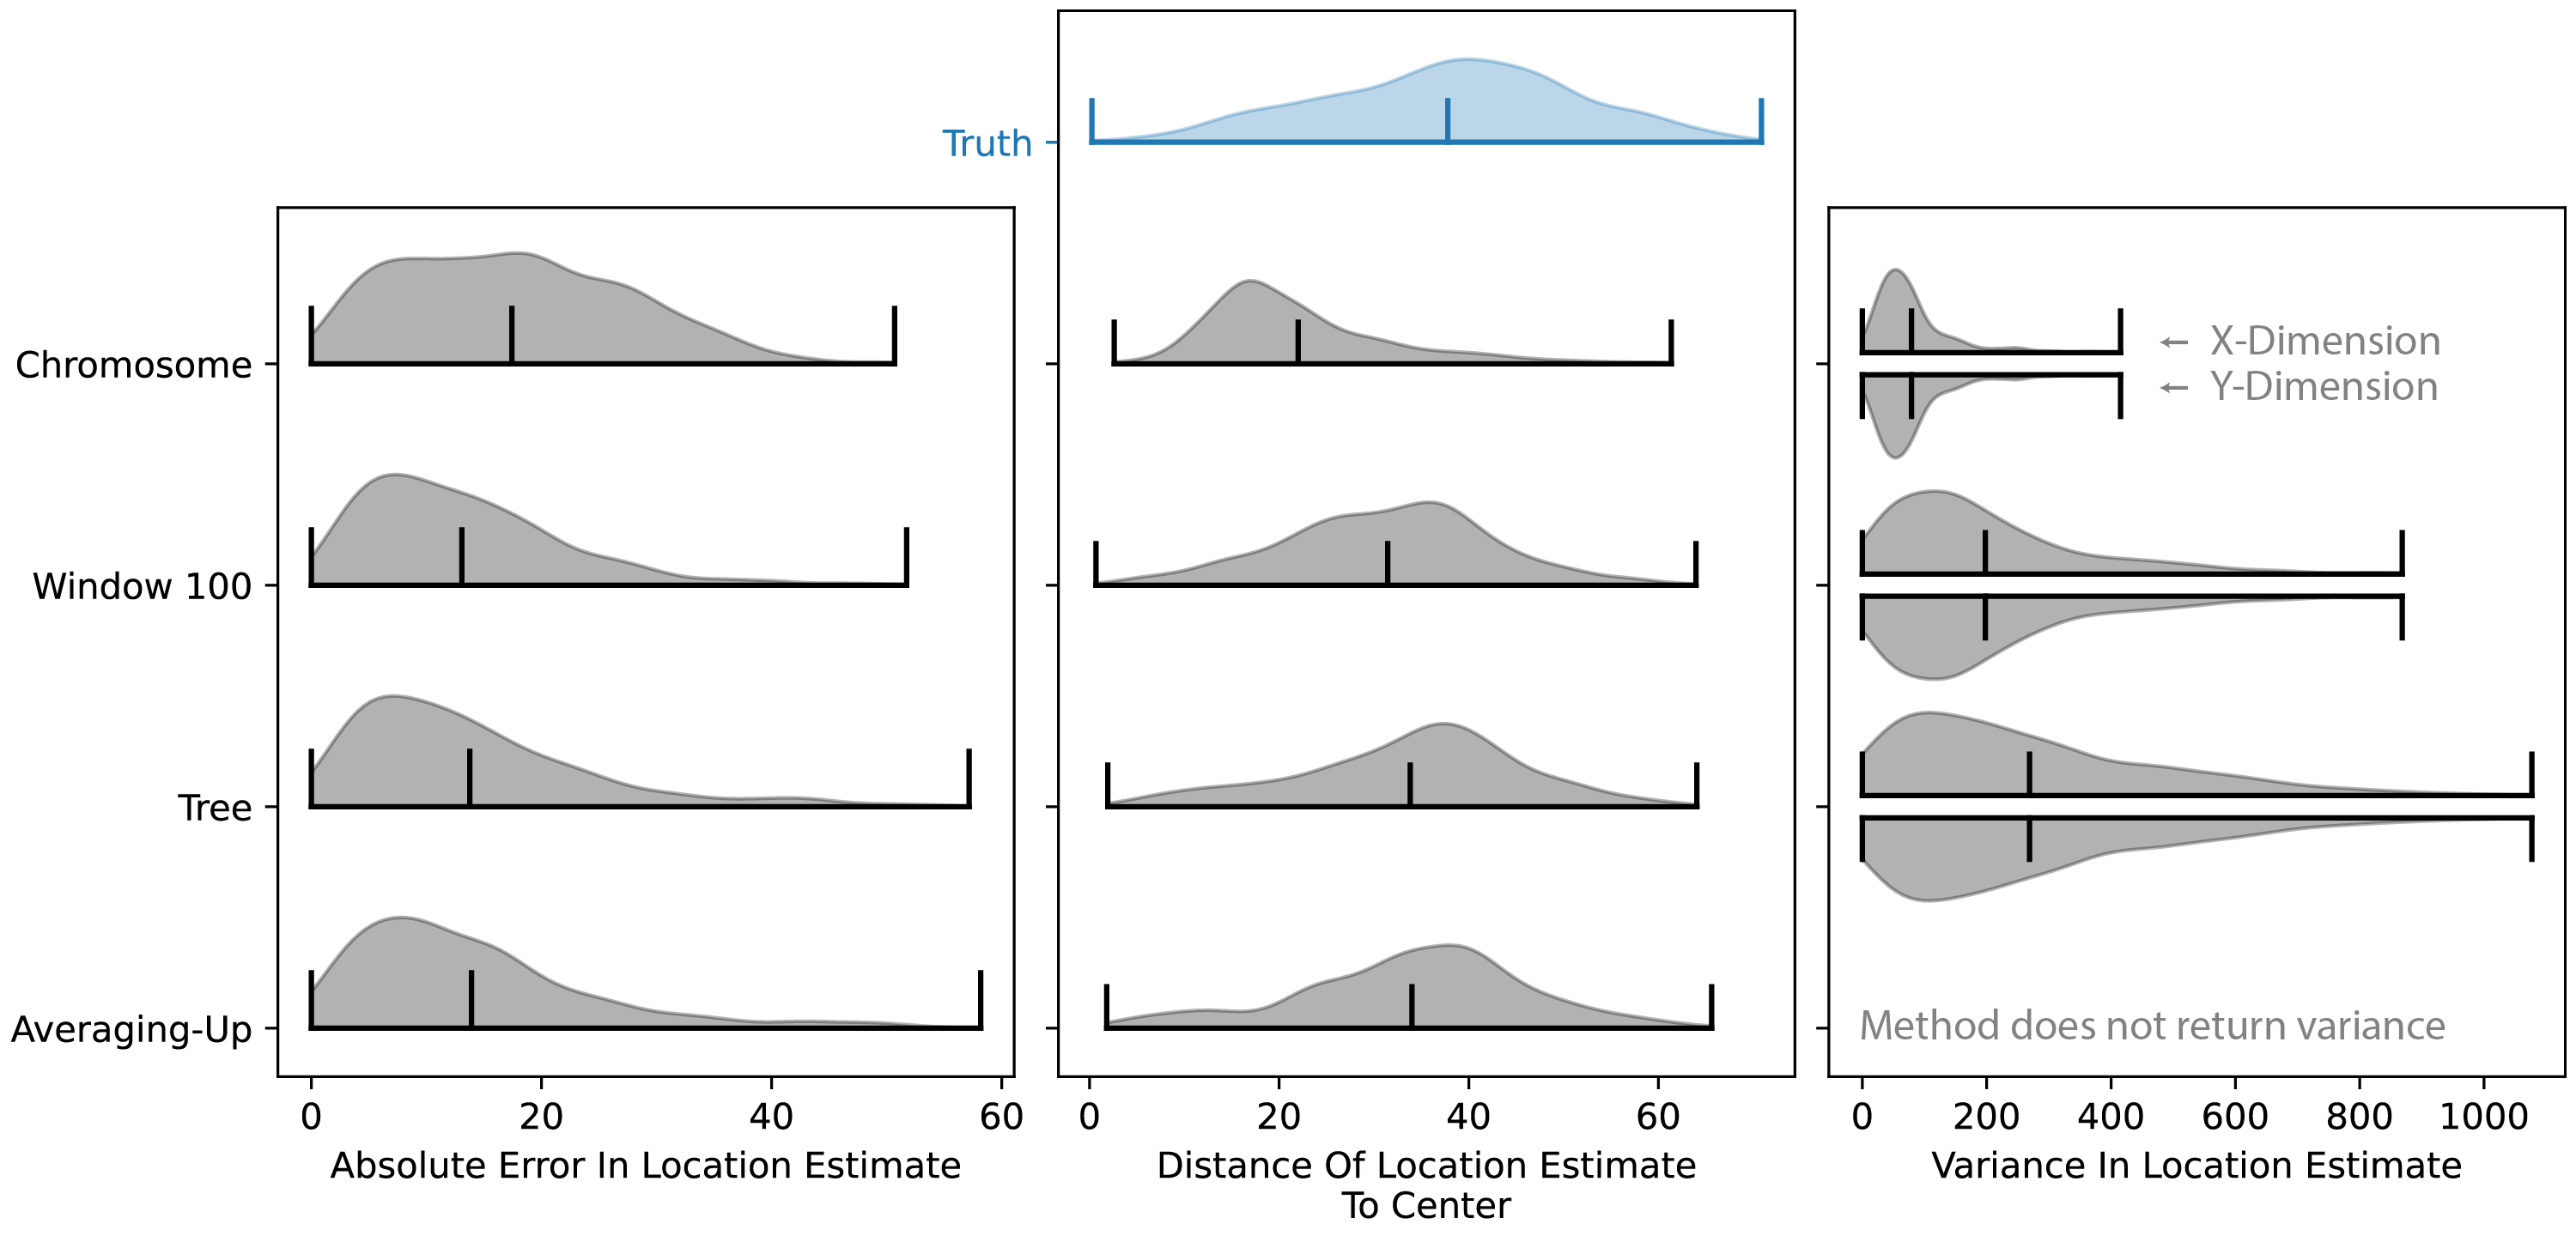
\includegraphics[width=425px]{Images/Figure6_LocationAccuracy/Fig6.png}
    \caption{\textbf{Accuracy of estimated ancestor locations}. (left) Distribution of distances between the MLE ancestor locations and their true locations. Horizontal lines show the extremes and mean of each distribution. (middle) Distributions of distances between the MLE ancestor locations and the average of the sample locations ("center"). The true distribution of distances of ancestor locations from the center is provided in blue for comparison. (right) Estimated variance in ancestor locations, computed using the effective dispersal rate from the simulation rather than the biased dispersal rate estimate.}
    \label{fig:ancestral_locations_plots}
\end{figure}

% The windowing approach reduces this bias while also providing a smaller variance in location estimates relative to W0, when using the local tree alone (\ref{fig:ancestral_locations_plots}B).
%We next estimated the variance in ancestor locations, using the true dispersal rate (since our estimated dispersal rates are biased). As described above for toy ARGs, using more information (trees) reduces our predicted uncertainty in ancestor locations (Figure \ref{fig:ancestral_locations_plots}B). Comparing the expected and observed coverage of confidence intervals, the higher variance from small window sizes overestimates uncertainty while the lower variance from large window sizes underestimates uncertainty (Figure \ref{fig:ancestral_locations_plots}C). Because our model is an approximation of the simulation, no window size perfectly estimates uncertainty. The averaging-up method does not provide a metric of uncertainty.  

\section{Promise of the approach}

Acknowledging the problems illustrated above, we would like to end by illustrating the goal and promise of using an ARG-based approach for spatial reconstruction. Recombinant chromosomes show an intricate pattern of splits and mergers with other samples as they move through time and space. For example, in an admixed individual, two regions of the chromosome will have identical spatial histories in the recent past, when they were inherited together, but very distinct spatial histories before they were brought together via recombination. To demonstrate this, we set up a simulation that starts with two geographically isolated subpopulations. Over 1000 generations, individuals in the two subpopulations disperse, meet, and interbreed. At the end of the simulation there is still a clear cline in genetic ancestry along the axis of separation between the original two subpopulations (Figure \ref{fig:tracking_recomb_sample}a). This cline was required for us to reconstruct the locations of genetic ancestors back to their original subpopulations. We then reconstructed the spatial histories of the chromosome regions on either side of a recombination event. We highlighted this breakpoint specifically because it separates genetic material from the two subpopulations, brought together 412 generations in the past. The ARG-based approach captured the "Y" pattern seen in the true locations, where following forward in time, the two lineages started in separate subpopulations before merging into a single path at the recombination event (Figure \ref{fig:tracking_recomb_sample}b). This pattern was not seen in estimates from individual trees as that approach does not take into account the sharing of edges between trees. Treating the two trees independently, the two lineages only come together at present day, where they meet at the sample.
Other ARG-based approaches to spatial inference \citep{Wohns2022,grundler2024} can also capture the splitting of lineages at recombination events, but do not provide measures of uncertainty, which hinders the development of hypothesis tests.




%One particularly promising application of our ARG-based inference is to locate recombination events, as well as the lineages involved in these events. This would, for example, allow us to more fully visualize the geographic history of admixed individuals. To demonstrate this, we set up a simulation that starts with two geographically isolated subpopulations. Over 1000 generations, individuals in the two subpopulations disperse and meet. At the end of the simulation there is still a clear cline in genetic ancestry along the axis of separation between the original two sub-populations (Fig \ref{fig:tracking_recomb_sample}A). This cline is required for us to reconstruct the locations of genetic ancestors back to their original subpopulations. If this cline did not exist, meaning that the two subpopulations have completely mixed, then there would not be a signal of the original subpopulation separation. We then reconstructed the spatial history of a sample on either side of a recombination event that splits the subpopulation it inherited genetic material from. Using our approach, we estimate the ancestral locations reasonably well and capture the fact that the two lineages were in the same location below the recombination event (Figure \ref{fig:tracking_recomb_sample}B). In contrast, when we locate the same ancestors using only a local tree for each lineage, we fail to capture the recent intertwined history or explicitly locate the recombination event.

%Treating the trees individually (e.g., using the method in \cite{Osmond2021}) fails to capture the fact that the movement of these lineages were completely  non-independent from each other in recent times. The blue and orange lines track the lineages of only two of the eight regions of the chromosome; the true locations of remaining six are shown in grey.

\begin{figure}
    \centering
    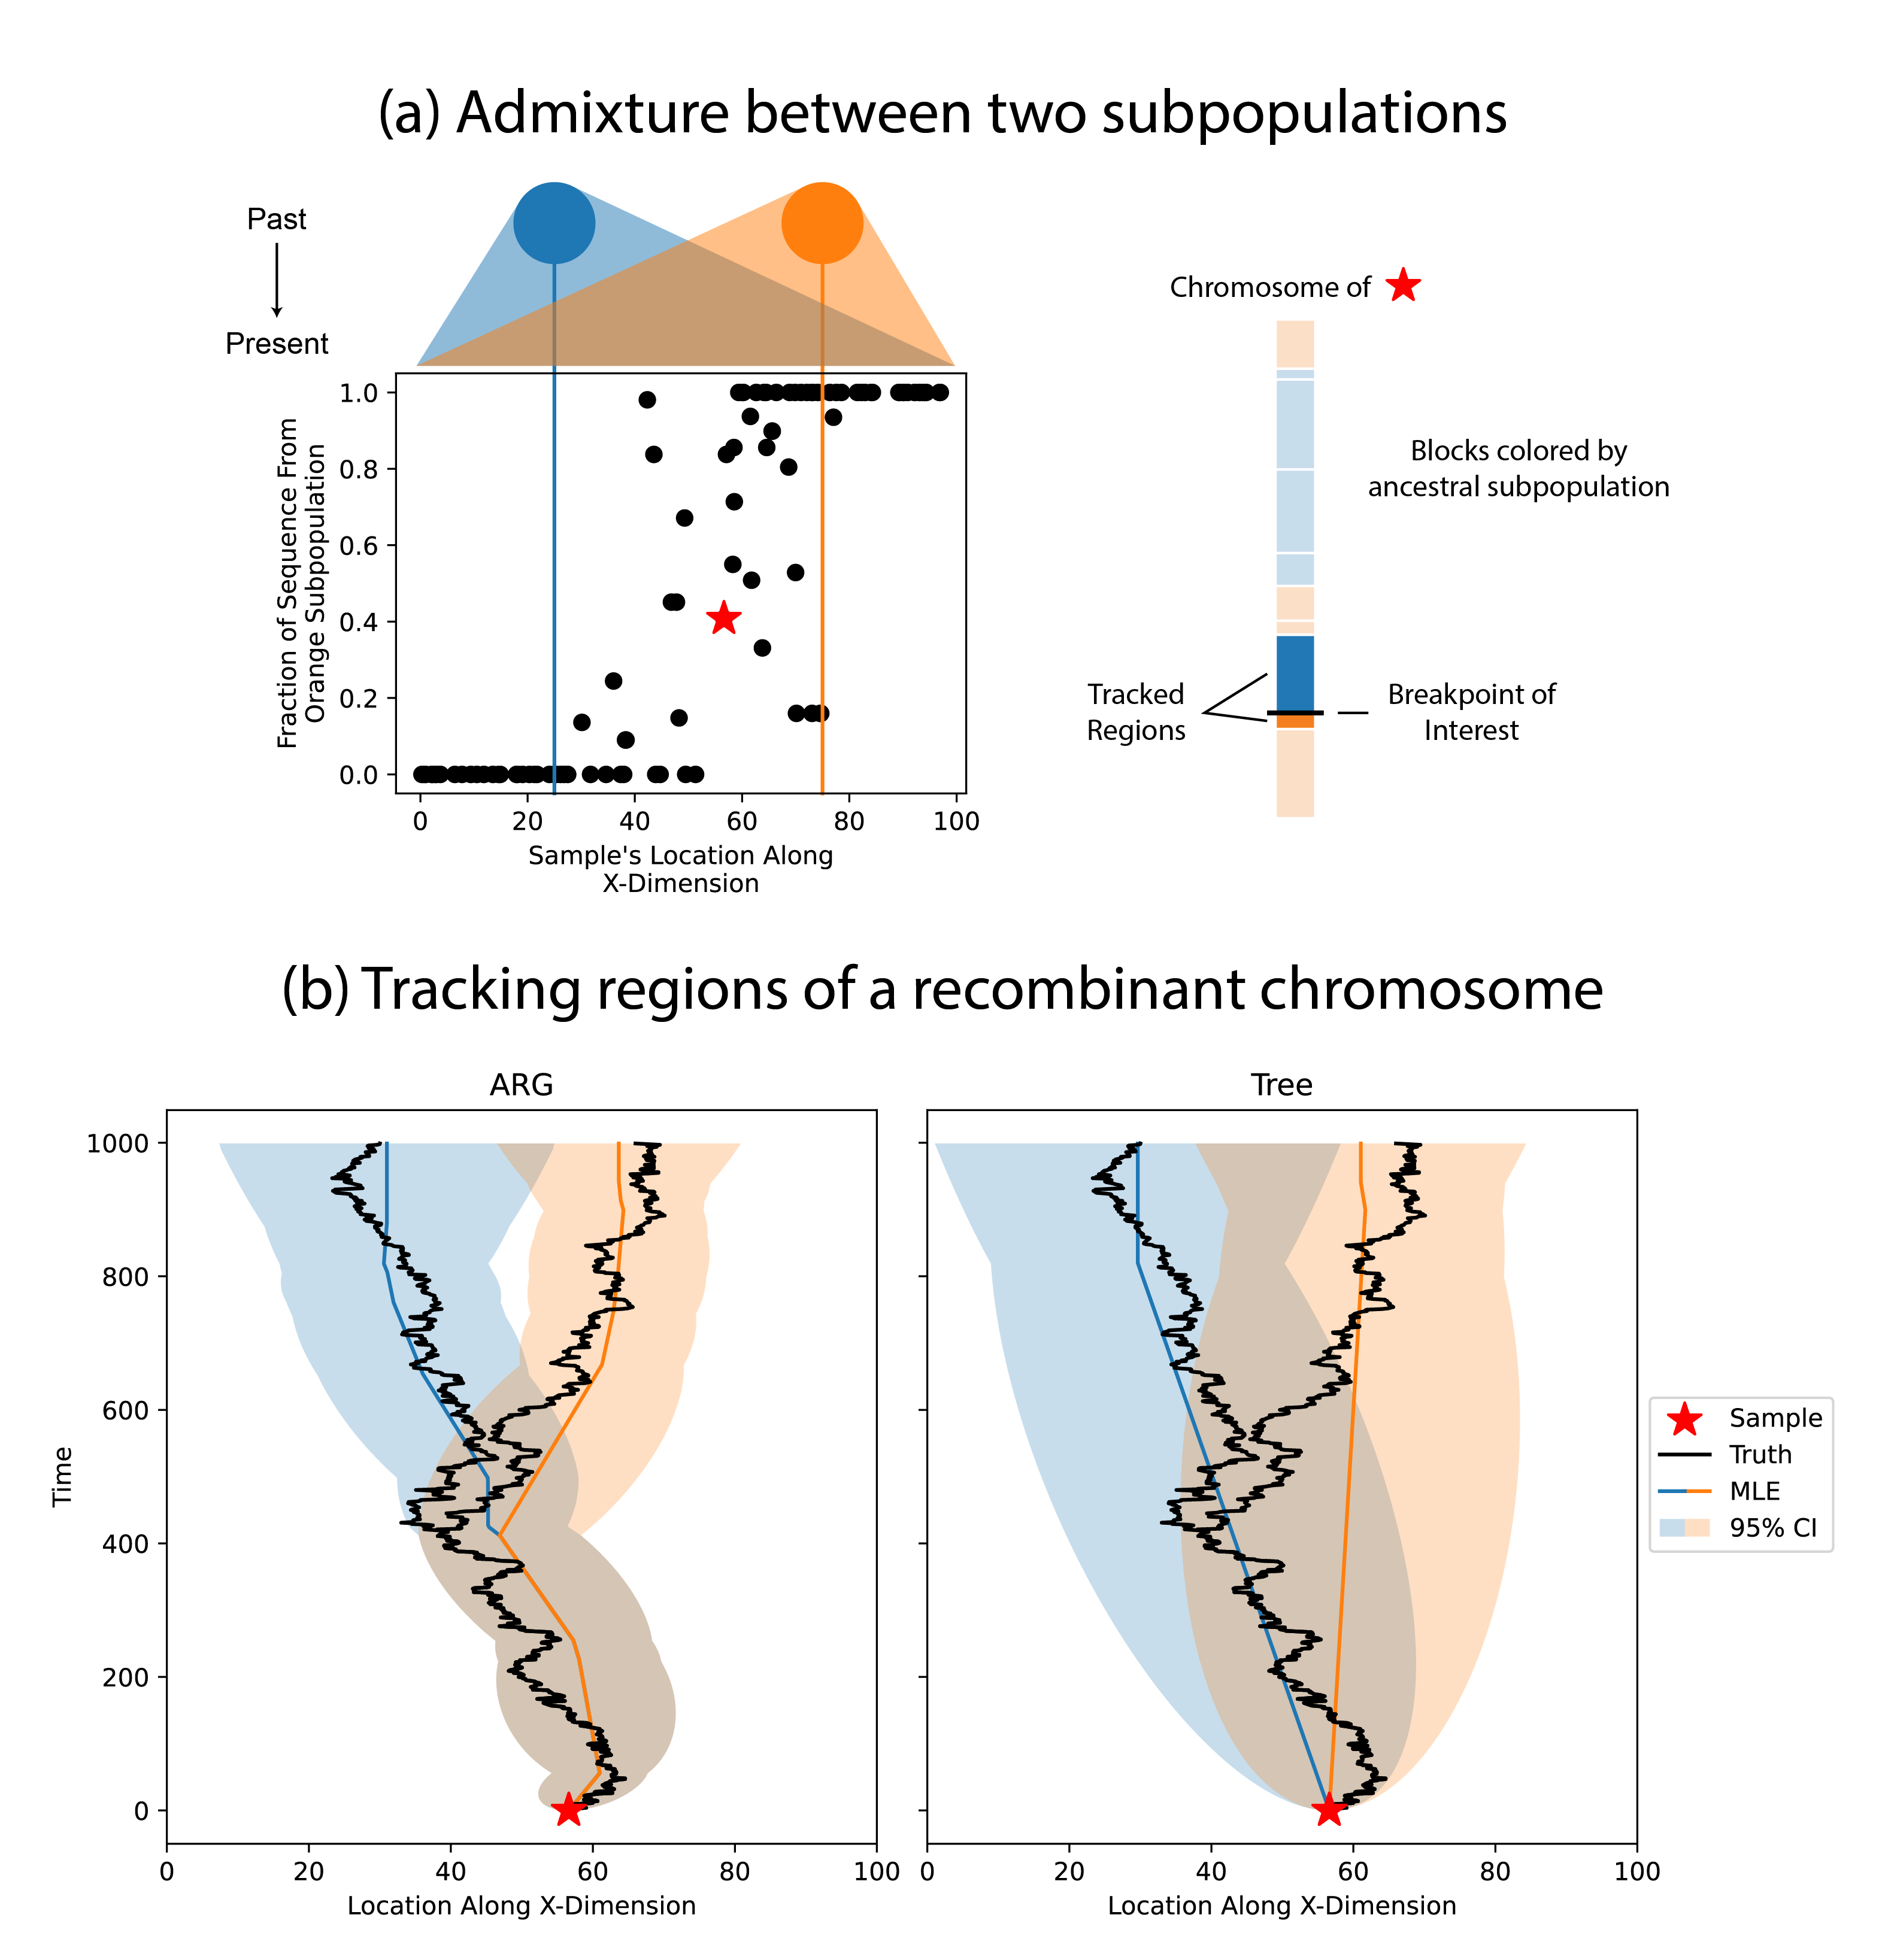
\includegraphics[width=400px]{Images/Figure7_TwoPop/Fig7_Complete_V2.png}
    \caption{\textbf{Visualizing the geographic history of admixture}. We simulated two geographically isolated subpopulations dispersing into one another, leading to samples with genetic ancestors from both subpopulations. (a) At the top of subfigure is a cartoon of the dispersion of the subpopulations over time. The colored vertical lines mark the average starting position of each subpopulation along the X-dimension. As you look at samples positioned from left to right, the fraction of their sequence associated with the orange subpopulation increases. Regions of the starred sample's chromosome are colored according to their associated ancestral subpopulation. The regions surrounding the breakpoint of interest are tracked in the following subfigure. (b) Two spatial reconstructions using the ARG for the full chromosome and the local trees on either side of the breakpoint. The black lines mark the true locations of the lineages, the colored lines are the estimated most likely ancestral locations, and the shading is the 95\% confidence interval around these estimates (using the effective dispersal rate from the SLiM simulation).
    }
    \label{fig:tracking_recomb_sample}
\end{figure}


\section{Data Availability}

Our method is available as a Python package at \url{https://github.com/osmond-lab/sparg}. The code for all of our analyses in this paper is available in the "manuscript" branch of the GitHub repository (\url{https://github.com/osmond-lab/sparg/tree/manuscript}).



\newpage



